\documentclass[12pt,a4paper]{article}
\usepackage[utf8]{inputenc}
\usepackage[english, greek, russian]{babel}
\usepackage{amsmath}
\usepackage{amsfonts}
\usepackage{array}
\usepackage{amssymb}
\usepackage{float}
\usepackage{makeidx}
\usepackage{geometry} 
	\geometry{top=30mm}
	\geometry{bottom=40mm}
	\geometry{left=25mm}
	\geometry{right=25mm}
\usepackage{hyperref}
\usepackage{wrapfig}
\usepackage[usenames,dvipsnames,svgnames,table,rgb]{xcolor}
\hypersetup{			
    unicode=true,           
    colorlinks=true,      
    linkcolor=black,          
    citecolor=black,       
    filecolor=magenta,      
    urlcolor=blue           
}
\usepackage{graphicx}
\author{Алексей Старченко \\ На основе материалов из \href{https://ru.wikipedia.org/wiki/\%D0\%A1\%D0\%BF\%D0\%B5\%D0\%BA\%D1\%82\%D1\%80\%D0\%B0\%D0\%BB\%D1\%8C\%D0\%BD\%D1\%8B\%D0\%B5_\%D0\%BA\%D0\%BB\%D0\%B0\%D1\%81\%D1\%81\%D1\%8B_\%D0\%B7\%D0\%B2\%D1\%91\%D0\%B7\%D0\%B4}{Википедии}}
\title{Спектральные классы звёзд}
\usepackage{wasysym}

\begin{document}
\maketitle

\tableofcontents \hspace{1pt}

\begin{wrapfigure}[9]{r}{0.5\textwidth}
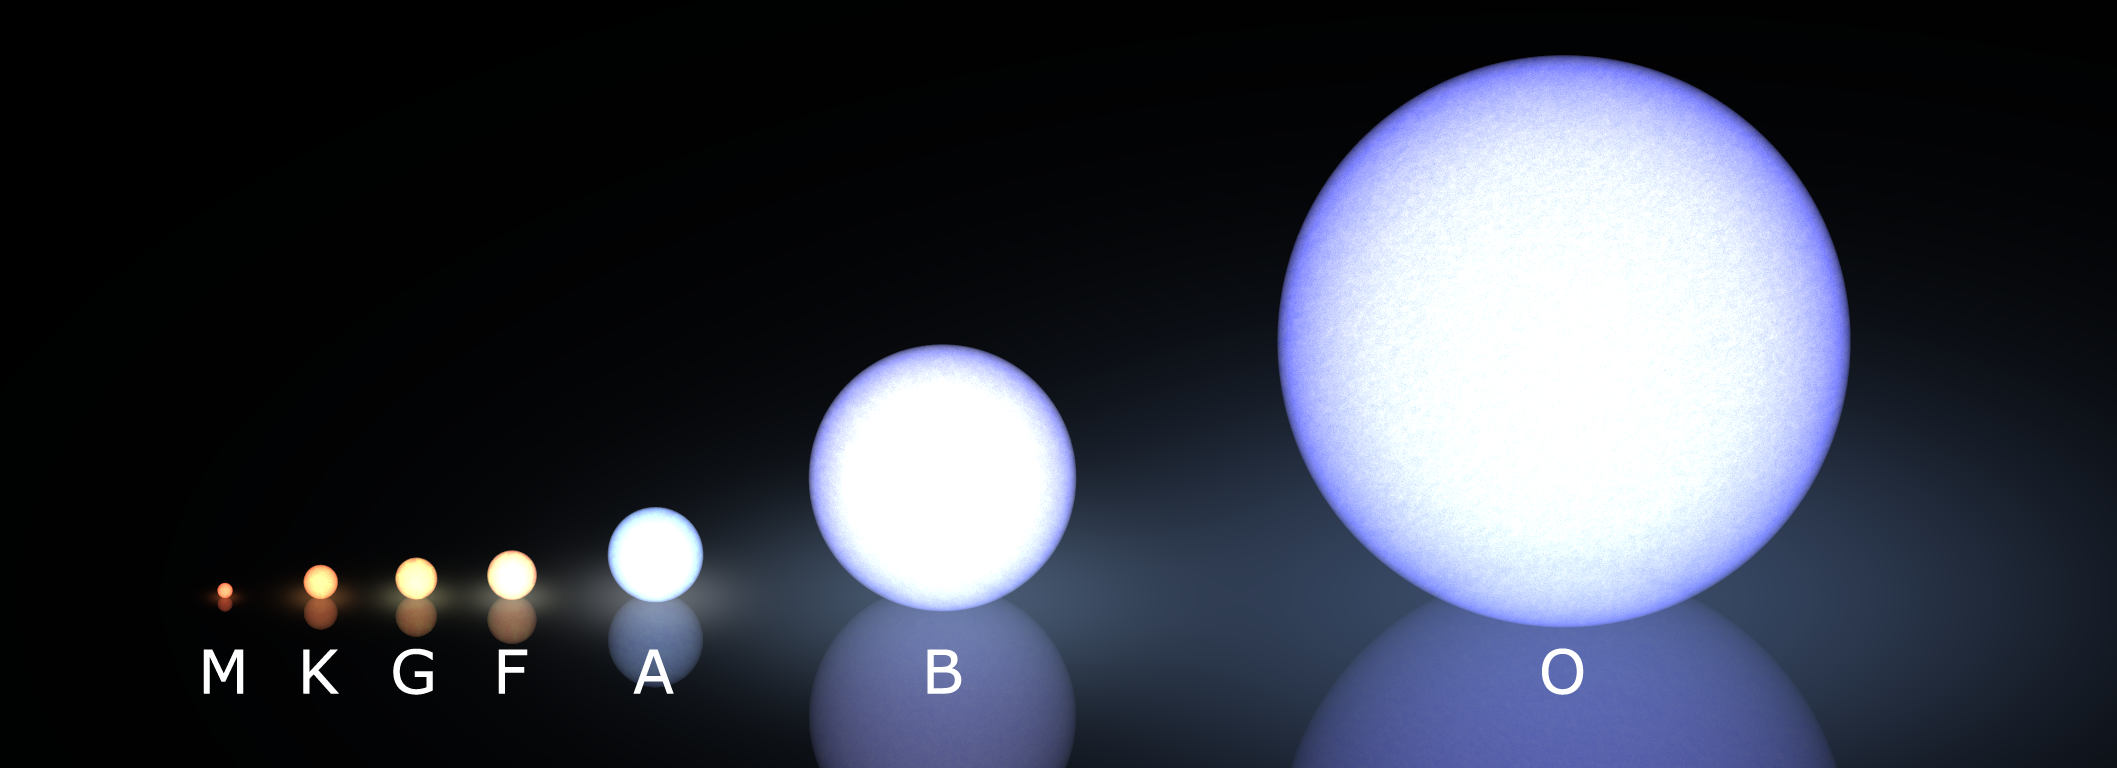
\includegraphics[scale=0.105]{1.png}
{\footnotesize Спектральная классификация Моргана-Кинана}
\end{wrapfigure} 


\textbf{Спектрaльные клaссы} -- классификация звёзд по спектру излучения, в первую очередь, по температуре фотосферы. Различия в спектрах звезд обусловливаются различием физических свойств их атмосфер, в основном, температуры и давления (определяющих степень ионизации атомов). Вид спектра зависит также от наличия магнитных и межатомных электрических полей, различий в химическом составе, вращения звезд и от других факторов.

Сплошной спектр излучения звезды близок к излучению абсолютно чёрного тела с температурой, равной температуре её фотосферы, которую можно оценить по закону смещения Вина, но для удалённых звёзд этот метод неприменим из-за неравномерного поглощения света различных участков спектра межзвёздной средой. Более точным методом является оптическая спектроскопия, позволяющая наблюдать в спектрах звёзд линии поглощения, имеющие различную интенсивность в зависимости от температуры и типа звезды. Для некоторых типов звёзд в спектрах наблюдаются и линии испускания.


\section{Классы Анджело Секки}
В 1860--1870-х годах пионер звёздной спектроскопии Анджело Секки создал первую классификацию звёздных спектров. В 1866 году он разбил наблюдаемые спектры звёзд на три класса в порядке убывания температуры поверхности звезды и соответствующего изменения цвета\cite{2}\cite{3}. В 1868 году Секки открыл углеродные звёзды, которые выделил в отдельную четвёртую группу\cite{4}. А в 1877 году он добавил пятый класс\cite{5}.

\begin{enumerate}
\item Класс I -- белые и голубые звезды с широкими линиями поглощения водорода в спектре, такие, как Вега и Альтаир; включает в себя современные класс A и начало класса F.
\begin{itemize}
\item Класс I, подтип Ориона -- звёзды класса I с узкими линиями в спектре вместо широких полос, такие, как Ригель и $\gamma$ Ориона; соответствует началу современного класса B.
\end{itemize}
\item Класс II -- жёлтые и оранжевые звёзды со слабыми линиями водорода, но с отчётливыми линиями металлов, такие, как Солнце, Арктур и Капелла; включает в себя современные классы G и К, а также конец класса F.
\item Класс III -- оранжевые и красные звёзды, в спектре которых линии образуют полосы, темнеющие в сторону синего, такие, как Бетельгейзе и Антарес; соответствует современному классу М.
\item Класс IV -- красные звёзды с сильными полосами и линиями углерода, углеродные звёзды.
\item Класс V -- звёзды с эмиссионными линиями, такие, как $\gamma$ Кассиопеи и $\beta$ Лиры.

\end{enumerate}






Позднее Эдуард Пикеринг изменил определение класса V, разделив его на горячие звёзды с эмиссионными линиями гелия, углерода и азота (звёзды Вольфа -- Райе) и планетарные туманности\cite{6}.

Предложенное Секки деление спектров было общепринятым вплоть до конца 1890-х годов, когда постепенно к середине XX века было заменено Гарвардской классификацией, которая описывается ниже\cite{6}\cite{7}.

\section{Основная (гарвардская) спектральная классификация}

Современная (гарвардская) спектральная классификация звёзд, разработанная в Гарвардской обсерватории в 1890--1924 годах является температурной классификацией, основанной на виде и относительной интенсивности линий поглощения и испускания спектров звёзд.

Внутри класса звёзды делятся на подклассы от 0 (самые горячие) до 9 (самые холодные). Солнце имеет спектральный класс G2 и эквивалентную температуру фотосферы 5780 K\cite{11}.

\begin{table}[H] \centering
Основная (гарвардская) спектральная классификация звёзд
\begin{tabular}{|c|c|c|c|c|c|}
\hline
Класс & Температура,K & Истинный цвет &	Видимый цвет\cite{8}\cite{9} & M\astrosun & R\astrosun \\
\hline
O & 30 000--60 000 & голубой & голубой & 60 & 15\\
\hline
B & 10 000--30 000 & бело-голубой & бело-голубой и белый & 18 & 7\\
\hline
A & 7500--10 000 & белый & белый & 3,1 & 2,1 \\
\hline
F & 6000--7500 & жёлто-белый & белый & 1,7 & 1,3 \\
\hline
G & 5000--6000 & жёлтый & жёлтый & 1,1 & 1,1 \\
\hline
K & 3500--5000 & оранжевый & желтовато-оранжевый & 0,8 & 0,9 \\
\hline
M & 2000--3500 & красный & оранжево-красный & 0,3 & 0,4 \\
\hline
\end{tabular}
\end{table}

\begin{center}
\begin{tabular}{|c|c|c|m{2cm}|m{2cm}|m{1.5cm}|}
\hline
Класс & Светимость, L\astrosun & Линии водорода& Доля* в глав. послед.,\% \cite{10} & Доля* нa ветв. бел.к.,\% \cite{10} &	Доля* гигантских,\% \cite{10}\\
\hline
O &1 400 000 & слабые & ~0,00003034 & - & -\\
\hline
B & 20 000 & средние & 0,1214 & 21,8750 & -\\
\hline
A & 80 & сильные & 0,6068 & 34,7222 & -\\
\hline
F & 6 & средние & 3,03398 & 17,3611 & 7,8740\\
\hline
G & 1,2 & слабые & 7,6456 & 17,3611 & 25,1969\\
\hline
K & 0,4 & очень слабые & 12,1359 & 8,6806 & 62,9921\\
\hline
M & 0,04 & очень слабые & 76,4563 & - & 3,9370\\
\hline
\end{tabular}
\end{center}



{\scriptsize * Примечание к таблице: Данные вычислены по количеству звёзд с абсолютной звёздной величиной более +16 в окрестностях Солнца в 10000 пк$^3$ (радиус 10,77 пк = 35,13 св. л.). Это позволяет воспроизвести приблизительную картину распределения звёзд по спектральным классам, хотя бы для звёзд на расстоянии от Галактического центра до Солнца. (Колонка Доля гигантских содержит Гигантов, Ярких гигантов и Сверхгигантов)\cite{10}}



\section{Йеркская классификация с учётом светимости (МКК)}

\begin{wrapfigure}{r}{0.45\textwidth}
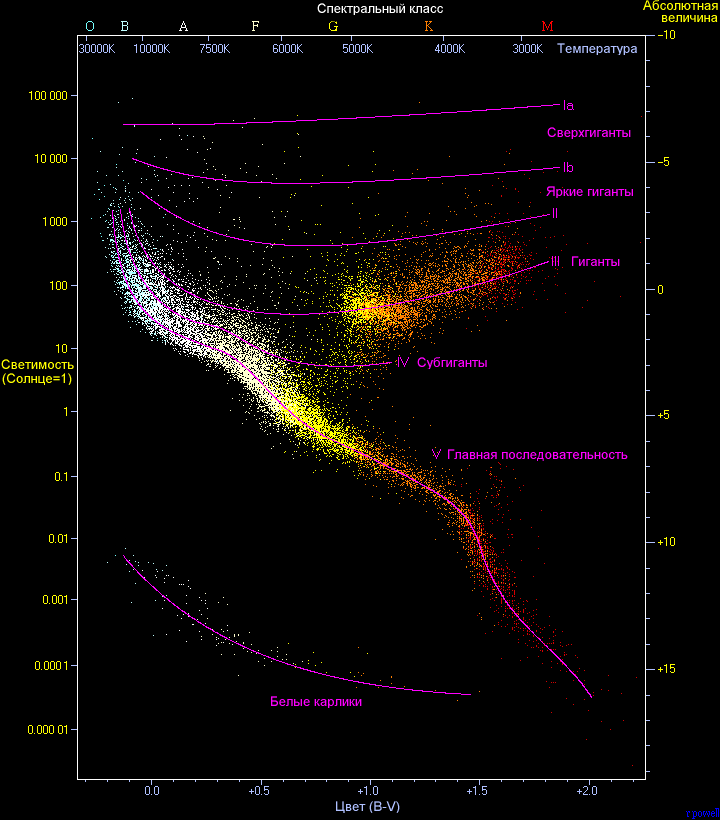
\includegraphics[scale=0.4]{2.png}
{\footnotesize Диаграмма спектральный класс—светимость (диаграмма Герцшпрунга -- Рассела)}
\end{wrapfigure}

Дополнительным фактором, влияющим на вид спектра, является плотность внешних слоёв звезды, зависящая, в свою очередь от её массы и плотности, то есть, в конечном итоге, от светимости. Особенно сильно зависят от светимости SrII, BaII, FeII, TiII, что приводит к различию в спектрах звёзд-гигантов и карликов одинаковых гарвардских спектральных классов.

Зависимость вида спектра от светимости отражена в более новой йеркской классификации, разработанной в Йеркской обсерватории (Yerkes Observatory) У. Морганом, Ф. Кинаном и Э. Келман, называемой также МКК по инициалам её авторов.

В соответствии с этой классификацией звезде приписывают гарвардский спектральный класс и класс светимости:
\begin{itemize}
\item Ia+ или 0 -- гипергиганты
\item I, Ia, Iab, Ib -- сверхгиганты
\item II, IIa, IIb -- яркие гиганты
\item III, IIIa, IIIab, IIIb -- гиганты
\item IV -- субгиганты
\item V, Va, Vb -- карлики (звезды главной последовательности)
\item VI -- субкарлики
\item VII -- белые карлики
\end{itemize}

Таким образом, если гарвардская классификация определяет абсциссу диаграммы Герцшпрунга -- Рассела, то йеркская -- положение звезды на этой диаграмме. Дополнительным преимуществом йеркской классификации является возможность по виду спектра звезды оценить её светимость и, соответственно, по видимой величине -- расстояние (метод спектрального параллакса).

Солнце, будучи жёлтым карликом, имеет йеркский спектральный класс G2V.

\section{Дополнительные спектральные классы}

Выделяют также дополнительные спектральные классы для некоторых классов небесных тел:

\begin{itemize}
\item W -- звёзды Вольфа -- Райе, очень тяжёлые яркие звёзды с температурой порядка 70000 K и интенсивными эмиссионными линиями в спектрах.
\item L -- звёзды или коричневые карлики с температурой 1500--2000 K и соединениями металлов в атмосфере.
\item T -- метановые коричневые карлики с температурой 700--1500 K.
\item Y -- очень холодные (метано-аммиачные) коричневые карлики с температурой ниже 700 K.
\item C -- углеродные звёзды, гиганты с повышенным содержанием углерода. Ранее относились к классам R и N.
\item S -- циркониевые звёзды
\item D -- белые карлики
\item Q -- новые звёзды
\item P -- планетарные туманности
\end{itemize}
\section{Характеристические особенности в классе}
У некоторых объектов могут наблюдаться дополнительные особенности в спектре. Чтобы указать на эти особенности к обозначению добавляют дополнительные префиксы и постфиксы.
\subsection{Добавочные индексы, стоящие перед обозначением спектра}
\begin{itemize}
\item d -- карлик (звезда главной последовательности)
\item esd -- экстремальный субкарлик
\item c -- сверхгигант
\item g -- гигант
\item sg -- субгигант
\item sd -- субкарлик
\item w или wd -- белый карлик
\end{itemize}
\subsection{Добавочные индексы, стоящие после обозначения спектра}
\begin{itemize}
\item c -- глубокие узкие линии
\item comp -- составной спектр
\item con -- отсутствуют видимые линии поглощения
\item e -- эмиссия (эмиссия водорода в O-звездах)
\item em -- эмиссия в линиях металлов
\item ep -- пекулярная эмиссия (линии, по своему характеру отличные от нормально соответствующих классу)
\item er -- явственно обращённые эмиссионные линии
\item eq -- эмиссия с поглощением на более коротких волнах
\item ev -- переменность относится только к эмиссионным линиям
\item ew -- эмиссии, типичные для звёзд класса W
\item f, (f), ((f)) -- эмиссия гелия и неона в O-звездах
\item h -- звёзды класса WR с эмиссионными линиями водорода
\item ha -- звёзды класса WR с эмиссионными линиями водорода как поглощения, так и излучения
\item k -- межзвёздные линии
\item m -- сильные линии металлов
\item n -- диффузные линии (широкие и размытые), обусловленные быстрым вращением
\item neb -- добавочный спектр туманности
\item nn -- очень размытые диффузные линии
\item p -- пекулярный спектр (имеются неправильности)
\item pq -- особенности напоминают спектр новой звезды
\item s -- резкие и узкие линии
\item sh -- наличие оболочки
\item ss -- очень узкие линии
\item v или var -- изменения в спектре (не обусловленные орбитальным движением и пульсацией)
\item w или wk или wl -- слабые линии
\end{itemize}


\section{Мнемоника}
Для запоминания основной последовательности гарвардской классификации существуют мнемонические формулы:

\begin{itemize}
\item на английском языке: Oh Be A Fine Girl, Kiss Me Right Now Sweetheart, а также множество других вариантов\cite{12}.
\item на русском языке: Один Бритый Англичанин Финики Жевал Как Морковь;
\item вариант, намекающий на Бориса Александровича Воронцова-Вельяминова: О, Борис Александрович Финики Жевал Как Морковь;
\item модификация, включающая классы W, R, N, S: Вообразите: Один Бритый Англичанин Финики Жевал Как Морковь -- Разве Не Смешно?;
\item О, Борис Александрович! Физики Ждут Конца Мучений (имеется в виду также Борис Александрович Воронцов-Вельяминов).
\item Также версия О. Н. Востряковой "ОБА Фраера Гуляют Как Могут.
\item Версия Ш. Т. Хабибуллина: О Боже, АФГанистан. Куда Мы Несемся. Эта мнемоника родилась задолго до войны в Афганистане (1966--1967, а возможно и раньше)
\end{itemize}

\addcontentsline{toc}{section}{Литература}
\begin{thebibliography}{99}


\bibitem{1}  Pietro Angelo Secchi. Analyse spectrale de la lumière de quelques étoiles, et nouvelles observations sur les taches solaires  // Comptes rendus hebdomadaires des séances de l’Académie des sciences. -- Juillet--Décembre 1866. -- Vol. 63. -- P. 364--368.  
\bibitem{2}  Pietro Angelo Secchi. Nouvelles recherches sur l'analrse spectrale de la lumière des étoiles  // Comptes rendus hebdomadaires des séances de l’Académie des sciences. -- Juillet--Décembre 1866. -- Vol. 63. -- P. 621--628. 
\bibitem{3}  J. B. Hearnshaw. The analysis of starlight: One hundred and fifty years of astronomical spectroscopy. -- Cambridge University Press, 1987. -- P. 62--63. -- 546 p. -- ISBN 0-521-25548-1, ISBN 978-0-521-25548-6..
\bibitem{4}  J. B. Hearnshaw. -- 1987. -- P. 62--63.
\bibitem{5}  J. B. Hearnshaw. -- 1987. -- P. 60.
\bibitem{6}  Перейти к: 1 2 James B. Kaler. Stars and their spectra: an introduction to the spectral sequence. -- Cambridge University Press, 1997. -- P. 62--63. -- 300 p. -- ISBN 0-521-58570-8, ISBN 978-0-521-58570-5..  
\bibitem{7}  Stephen Gottesman. Classification of stellar spectra: Some history  (4 February 2004). 
\bibitem{8}  The Guinness book of astronomy facts \& feats, Patrick Moore, 1992, 0-900424-76-1
\bibitem{9}  The Colour of Stars. Australia Telescope Outreach and Education (December 21 2004). -- Explains the reason for the difference in color perception.
\bibitem{10}  Перейти к: 1 2 3 4 LeDrew, G.; The Real Starry Sky, Journal of the Royal Astronomical Society of Canada, Vol. 95, No. 1 (whole No. 686, February 2001), pp. 32–33. Примечание: Таблица 2 содержит ошибку и для подсчёта звёзд главной последовательности, белых карликов и гигантских использовалось общее количество звёзд 824,00025 и 288 и 6,35 соответственно, а не 800 и 200 и 6,3 соответственно.
\bibitem{11}  Солнце // Физика космоса / под редакцией Р. А. Сюняева. -- 2-е изд. -- М.: Советская энциклопедия, 1986. -- С. 37.
\bibitem{12}  Allen S. J. Mnemonics for the Harvard Spectral Classification Scheme . UCL Astrophysics Group. 
\end{thebibliography}

\end{document}